\documentclass[t,aspectratio=169,11pt]{beamer}
\usepackage{fontspec}
\usefonttheme{professionalfonts}
\setmainfont{Noto Sans}\setsansfont{Noto Sans}\setmonofont{DejaVu Sans Mono}
\usepackage{amsmath,booktabs,graphicx,tikz}
\def\slideContentLeftMargin{0.65cm}
\def\slideContentRightMargin{0.65cm}
\def\hustHeaderHeight{1.0cm}
\usepackage[red,169]{hust/beamerthemeHUST}
\graphicspath{{hust/images/}{../artifacts/figures/}{../artifacts/screenshots/}}
% Điền thông tin nhóm tại đây; file này dùng chung cho report và slide.
\newcommand{\ProjectName}{ResearchLens}
\newcommand{\ProjectSubtitle}{Intelligent Research Paper Search and Discovery System}
\newcommand{\CourseName}{IT4868E -- Web Mining}
\newcommand{\Semester}{2026.1}
\newcommand{\TeamName}{Nhóm ResearchLens}
\newcommand{\TeamMembers}{Thông tin thành viên và MSSV: bổ sung trước khi nộp}
\newcommand{\Instructor}{TS. Nguyễn Kiêm Hiếu}
\newcommand{\ReportDate}{14 tháng 10 năm 2026}

\newcommand{\CatalogCount}{129.596}
\newcommand{\CatalogLatencyMedian}{44.2}
\newcommand{\CatalogLatencyTail}{153.2}
\newcommand{\CatalogBuildSeconds}{7.7}
\newcommand{\CatalogIndexMiB}{525.9}
\newcommand{\CatalogAbstractPercent}{73.1}

\definecolor{ink}{HTML}{172B3A}\definecolor{muted}{HTML}{65737C}
\setbeamercolor{normal text}{fg=ink,bg=white}
\setbeamercolor{itemize item}{fg=hustprimary}
\setbeamerfont{normal text}{size=\normalsize}
\setbeamerfont{frametitle}{size=\large,series=\bfseries}
\setbeamertemplate{frametitle}{\begin{tikzpicture}[remember picture,overlay]\node[anchor=west,xshift=.45cm,yshift=-.46cm,text width=15cm] at (current page.north west) {\color{white}\fontsize{15}{17}\selectfont\bfseries\insertframetitle};\end{tikzpicture}}
\setbeamertemplate{footline}{\hfill\raisebox{.17cm}{\color{muted}\fontsize{6}{7}\selectfont\insertsection\hspace{1.1cm}}}
\setbeamertemplate{navigation symbols}{}
\useStyleFull\showPageNumber
\setlength{\parskip}{5pt}
\newcommand{\source}[1]{\par\par\vspace{.1cm}{\fontsize{6.5}{8}\selectfont\color{muted}#1\par}}
\newcommand{\takeaway}[1]{\par{\color{hustprimary}\bfseries #1\par}}
\newcommand{\bigmetric}[2]{{\fontsize{32}{36}\selectfont\bfseries\color{hustprimary}#1\par}{\small #2\par}}
\newcommand{\chartslide}[4]{\begin{frame}{#1}\begin{columns}[T,onlytextwidth]\column{.69\textwidth}\includegraphics[width=\linewidth,height=5.35cm,keepaspectratio]{#2}\column{.27\textwidth}\raggedright\par\vspace{.35cm}#3\end{columns}\source{#4}\end{frame}}
\title{ResearchLens}\subtitle{\ProjectSubtitle}\author{\TeamName}\institute{\CourseName\quad /\quad Học kỳ \Semester}
\hypersetup{pdftitle={ResearchLens — Web Mining Capstone},pdfauthor={ResearchLens project team}}
\begin{document}
% Cover retains the original HUST template background and adds project-specific text.
{\setbeamertemplate{background}{
\includegraphics[width=\paperwidth,height=\paperheight]{hust-red-169-title.png}}\setbeamertemplate{headline}{}\setbeamertemplate{footline}{}
\begin{frame}[plain]
\begin{tikzpicture}[remember picture,overlay]
\node[anchor=west,text width=10.6cm] at ([xshift=.75cm,yshift=-.25cm]current page.west) {\color{hustprimary}\fontsize{34}{39}\selectfont\bfseries ResearchLens\par\par\vspace{.3cm}{\fontsize{15}{20}\selectfont\color{ink}Intelligent Research Paper\par Search and Discovery System\par}\par\vspace{.6cm}{\fontsize{10}{14}\selectfont\color{ink}\CourseName\quad ·\quad Học kỳ \Semester\par\TeamName\par}\par\vspace{.3cm}{\fontsize{8}{11}\selectfont\color{muted}\ReportDate\par}};
\end{tikzpicture}
\end{frame}}
\section{Bài toán}
\begin{frame}{Từ các bài đã lưu, gợi ý bài nên đọc tiếp}
\begin{columns}[T,onlytextwidth]
\column{.62\textwidth}
\par\vspace{.45cm}
{\Large Đã lưu vài bài. Đọc bài nào tiếp?}\par\par\vspace{.4cm}
\begin{enumerate}
\item[RQ1] Tín hiệu nào tìm lại tốt nhất: popularity, nội dung, PageRank cá nhân hóa hay đồng trích dẫn?
\item[RQ2] Kết hợp các tín hiệu có vượt tín hiệu tốt nhất?
\end{enumerate}
\column{.32\textwidth}
\par\vspace{.4cm}
\takeaway{Trọng tâm capstone}\par
Recommendation\par Link analysis
\par\vspace{.25cm}
{\small Review là bằng chứng cạnh gợi ý.\par Search là cách lưu bài đầu tiên.}
\end{columns}
\source{Nguồn yêu cầu: 20261\_syllabus.pdf; ResearchLens\_Visual\_Spec.pdf.}
\end{frame}
\section{Dữ liệu và thiết kế}
\begin{frame}{Snapshot đáp ứng phạm vi 2k--5k bài của đặc tả}
\begin{columns}[T,onlytextwidth]
\column{.3\textwidth}\bigmetric{3.595}{paper thật}\par\vspace{.35cm}\small 3.171 OpenAlex\par 424 PeerRead thêm mới
\column{.3\textwidth}\bigmetric{13.481}{cạnh citation nội bộ}\par\vspace{.35cm}\small 770 nút cô lập\par Graph có hướng
\column{.3\textwidth}\bigmetric{1.320}{scored reviews duy nhất}\par\vspace{.35cm}\small Giảm từ 2.642 bản\par Khử trùng trước train/test
\end{columns}
\par\vspace{.65cm}
\takeaway{Lưu cache, commit nguồn và SHA-256 để tái lập.}
\source{OpenAlex API; PeerRead (Kang et al., 2018), ICLR 2017. Snapshot 14/10/2026. Tám query relevance-ranked; không phải mẫu đại diện toàn bộ AI/ML.}
\end{frame}
\begin{frame}{Một pipeline CPU nối dữ liệu đến bằng chứng}
\par\vspace{.05cm}
\includegraphics[width=\textwidth,height=5.5cm,keepaspectratio]{architecture.pdf}
\source{Sơ đồ từ kiến trúc triển khai. Apache Solr 9.9.0 là backend tùy chọn đã index đủ 3.595 paper.}
\end{frame}
\begin{frame}{Người dùng kiểm tra được nguồn và tín hiệu xếp hạng}
\begin{columns}[T,onlytextwidth]\column{.76\textwidth}
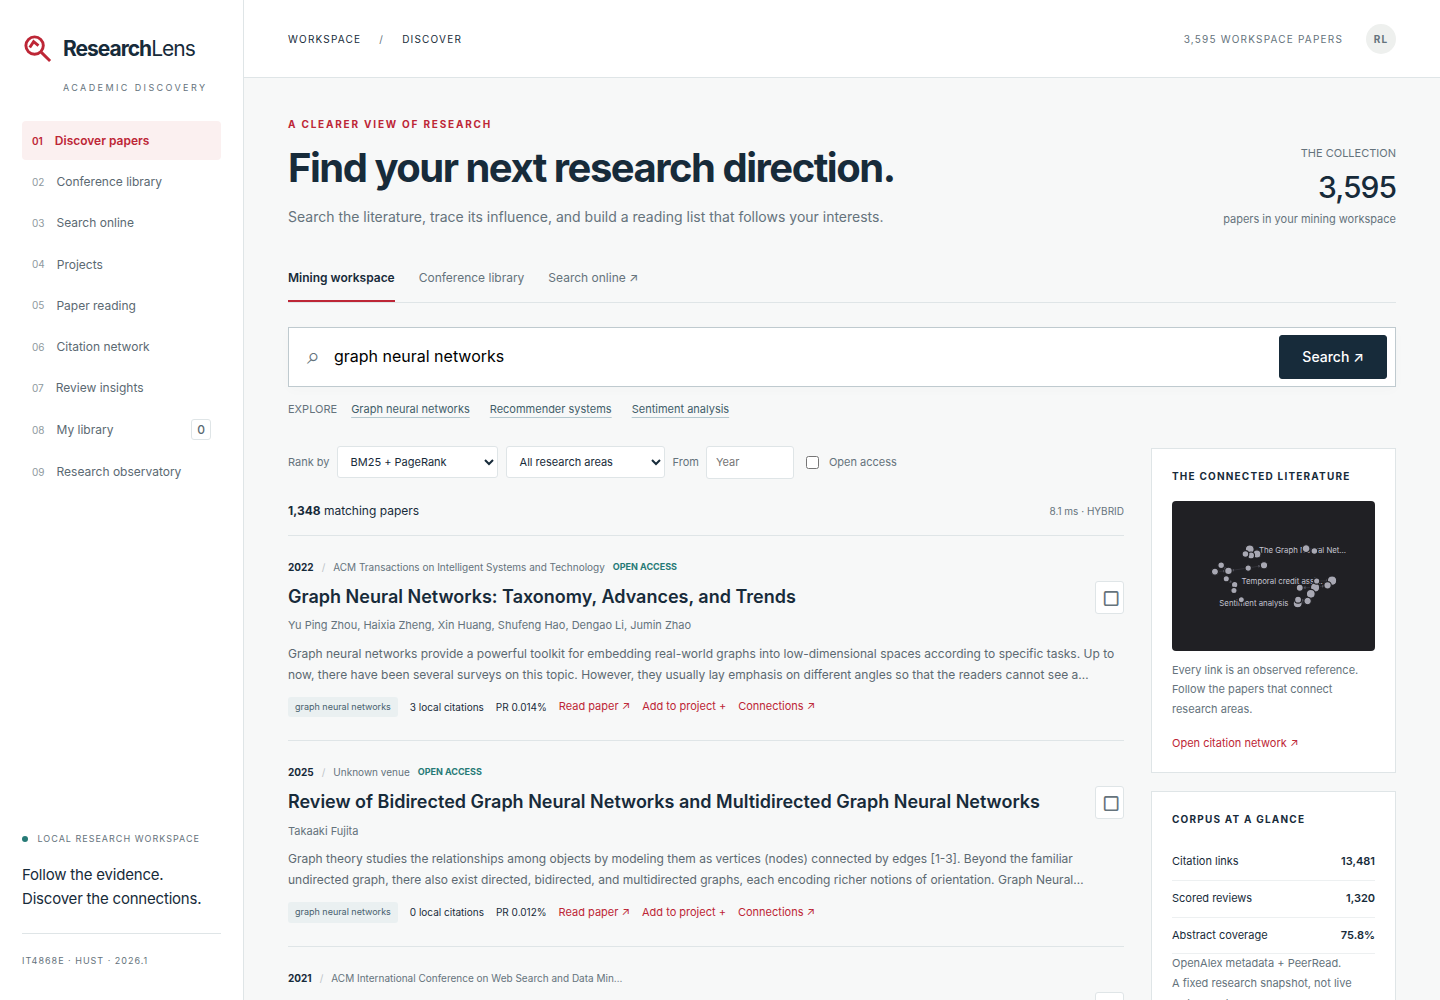
\includegraphics[width=\linewidth,height=5.55cm,keepaspectratio]{discover.png}
\column{.2\textwidth}\par\vspace{.4cm}\small
Query và bộ lọc\par\par\vspace{.3cm}
BM25 / TF-IDF / graph\par\par\vspace{.3cm}
Paper, nguồn, abstract\par\par\vspace{.3cm}
Lưu vào thư viện
\end{columns}
\source{Ảnh giao diện thật, chạy từ corpus bàn giao.}
\end{frame}
\begin{frame}{Kho hội nghị và benchmark có phạm vi riêng}
\begin{columns}[T,onlytextwidth]
\column{.73\textwidth}\includegraphics[width=\linewidth,height=5.25cm,keepaspectratio]{conference_coverage.pdf}
\column{.23\textwidth}\par\vspace{.4cm}{\fontsize{24}{28}\selectfont\bfseries\color{hustprimary}\CatalogCount\par}{\small bản ghi đã thu thập\par}\par\vspace{.4cm}\small 8 hội nghị\par 2020--2026\par\vspace{.25cm}FTS5 / BM25\par p95: \CatalogLatencyTail{} ms
\end{columns}
\source{Manifest crawl và catalog\_results.json; 100 warm query runs, không gồm HTTP. Coverage không phải tổng accepted papers. Các ô 0 là nguồn chưa có bản ghi.}
\end{frame}
\begin{frame}{Paper ngoài kho có thể tìm online rồi đưa vào Project}
\begin{columns}[T,onlytextwidth]
\column{.73\textwidth}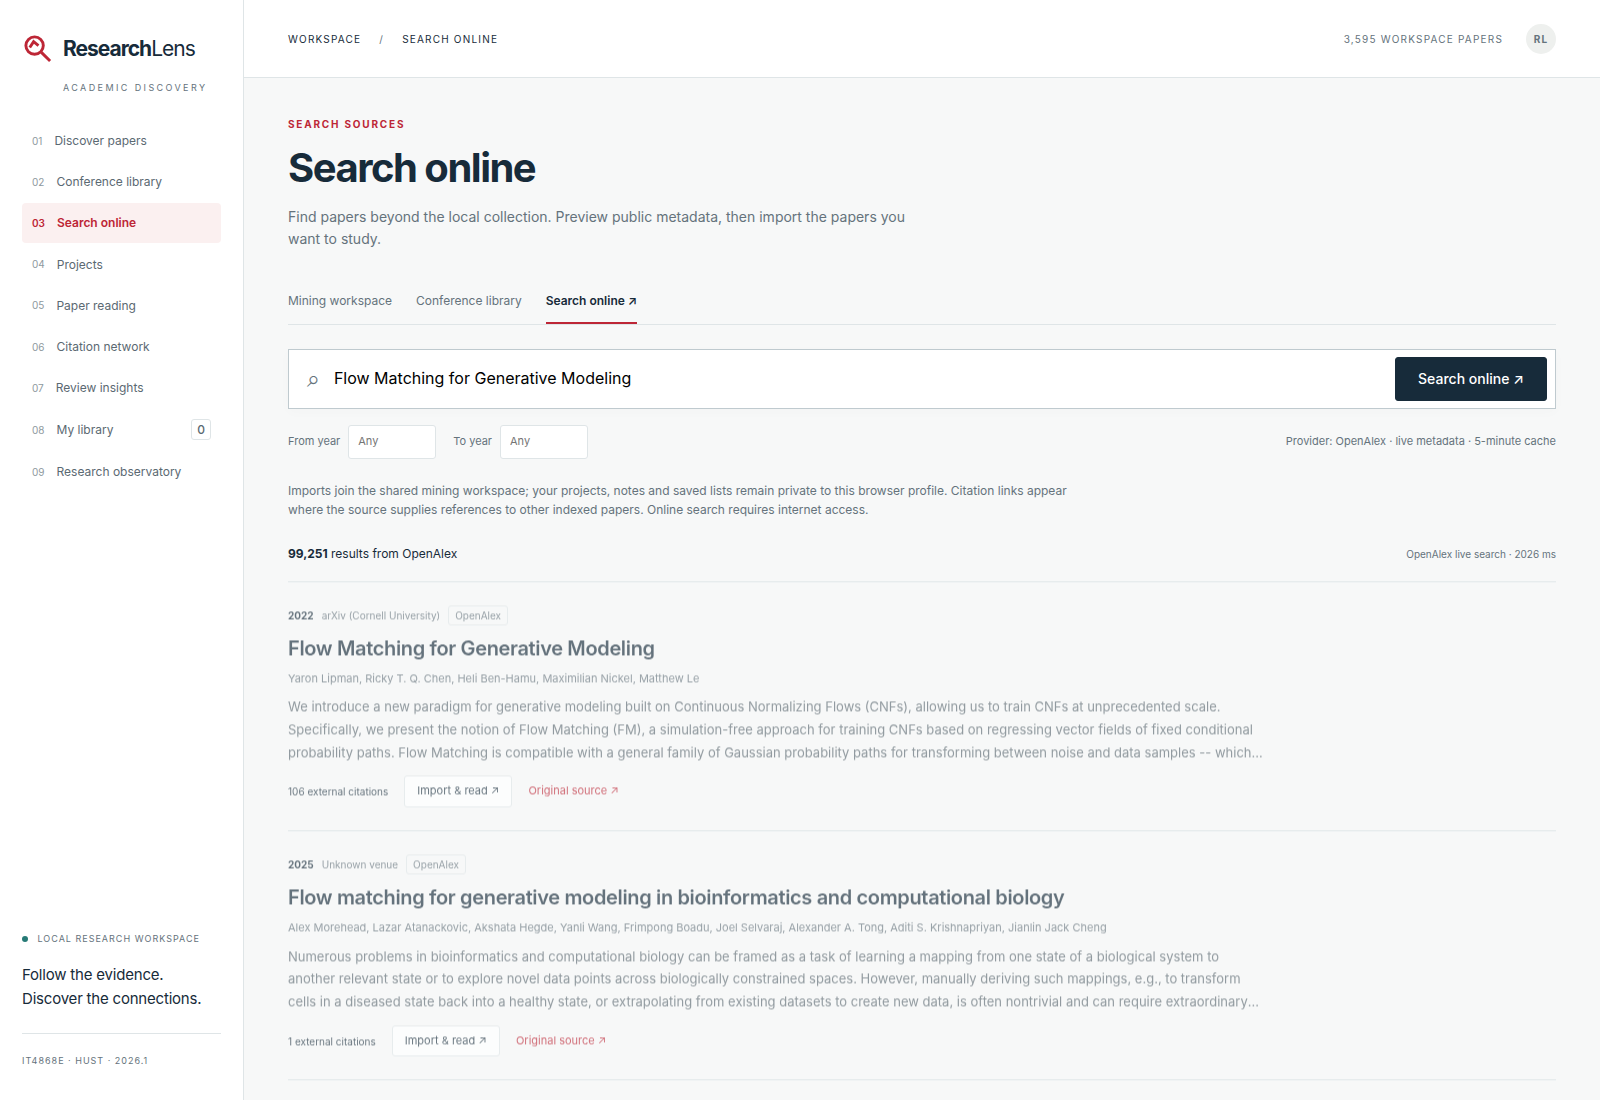
\includegraphics[width=\linewidth,height=5.5cm,keepaspectratio]{online_search.png}
\column{.23\textwidth}\par\vspace{.3cm}\small
OpenAlex live search\par\vspace{.3cm}
Import có khử trùng\par\vspace{.3cm}
Reader + Project\par\vspace{.3cm}
Alias nối citation\par\vspace{.3cm}
\takeaway{Nguồn thật; thiếu reference thì không tạo cạnh.}
\end{columns}
\source{Ảnh browser thật; import lưu vào corpus chung, notes/project riêng theo profile. Benchmark cũ không đổi sau import.}
\end{frame}
\section{Phương pháp}
\begin{frame}{Citation đi từ bài trích dẫn đến bài được trích dẫn}
\begin{columns}[T,onlytextwidth]
\column{.66\textwidth}\includegraphics[width=\linewidth,height=5.1cm,keepaspectratio]{network.pdf}
\column{.3\textwidth}\par\vspace{.3cm}
\textbf{PageRank}\par\small Độ ảnh hưởng nội bộ.
\par\vspace{.2cm}\par\normalsize\textbf{HITS}\par\small Authority và hub.
\par\vspace{.2cm}\par\normalsize\textbf{Louvain}\par\small Cộng đồng trên projection vô hướng.
\end{columns}
\source{Page et al. (1999); Kleinberg (1999); Blondel et al. (2008). Hình: 160 nút PageRank cao nhất, cạnh thật.}
\end{frame}
\begin{frame}{Hybrid kết hợp hồ sơ nội dung với citation proximity}
\par\vspace{.3cm}
\[
 s(d\mid S)=0.7\widehat{\cos}(d,S)+0.3\widehat{\mathrm{PPR}}(d\mid S)
\]
\par\vspace{.35cm}
\begin{columns}[T,onlytextwidth]
\column{.46\textwidth}\textbf{Hồ sơ}\par Trung bình TF-IDF của bài đã lưu.\par Restart PageRank trên seed.
\column{.46\textwidth}\textbf{Danh sách}\par Loại seed khỏi ứng viên.\par MMR giảm lặp nội dung.
\end{columns}
\par\vspace{.4cm}\takeaway{Weights cố định; chưa tune trên test.}
\source{Page et al. (1999); Carbonell \& Goldstein (1998). MMR: 150 ứng viên đầu, diversity penalty 0,15.}
\end{frame}
\begin{frame}{Mặc định: ghép hạng đồng trích dẫn với hạng hybrid}
\par\vspace{.3cm}
\[
 s_{\mathrm{fusion}}(d\mid S)=\frac{1}{60+r_{\mathrm{hybrid}}(d)}+\frac{\mathbf{1}[d\text{ có phiếu}]}{60+r_{\mathrm{co\text{-}cite}}(d)}
\]
\par\vspace{.35cm}
\begin{columns}[T,onlytextwidth]
\column{.46\textwidth}\textbf{Đồng trích dẫn}\par Bài $w$ trích cả $d$ và một bài đã lưu thì $d$ được một phiếu.\par Người dùng mở được bài $w$.
\column{.46\textwidth}\textbf{Vì sao dùng hạng}\par Phiếu và điểm hybrid khác thang đo.\par Bài chưa ai trích cùng vẫn có hạng hybrid.
\end{columns}
\par\vspace{.4cm}\takeaway{$k=60$ lấy từ bài gốc, không chỉnh trên dữ liệu dự án.}
\source{Small (1973); Cormack, Clarke \& Buettcher (2009), reciprocal rank fusion.}
\end{frame}
\begin{frame}{Review mining giữ câu gốc bên cạnh dự đoán}
\begin{columns}[T,onlytextwidth]
\column{.53\textwidth}
\par\vspace{.3cm}\textbf{Bộ phân loại}\par TF-IDF unigram/bigram\par Logistic regression, $C=1$\par Train-only vocabulary
\par\vspace{.3cm}\small Nhãn: $r\leq4$ critical; 5--6 mixed; $r\geq7$ positive.
\column{.41\textwidth}\par\vspace{.3cm}\textbf{Evidence theo khía cạnh}\par Novelty · Soundness\par Evaluation · Clarity\par Reproducibility
\par\vspace{.3cm}\takeaway{Rating là nhãn proxy, không phải verdict chất lượng.}
\end{columns}
\source{PeerRead: Kang et al. (2018). Aspect keywords + lexicon là heuristic, chưa có gold aspect benchmark.}
\end{frame}
\section{Workspace nghiên cứu}
\begin{frame}{Brief, paper và citation map nằm trong một Project}
\begin{columns}[T,onlytextwidth]
\column{.73\textwidth}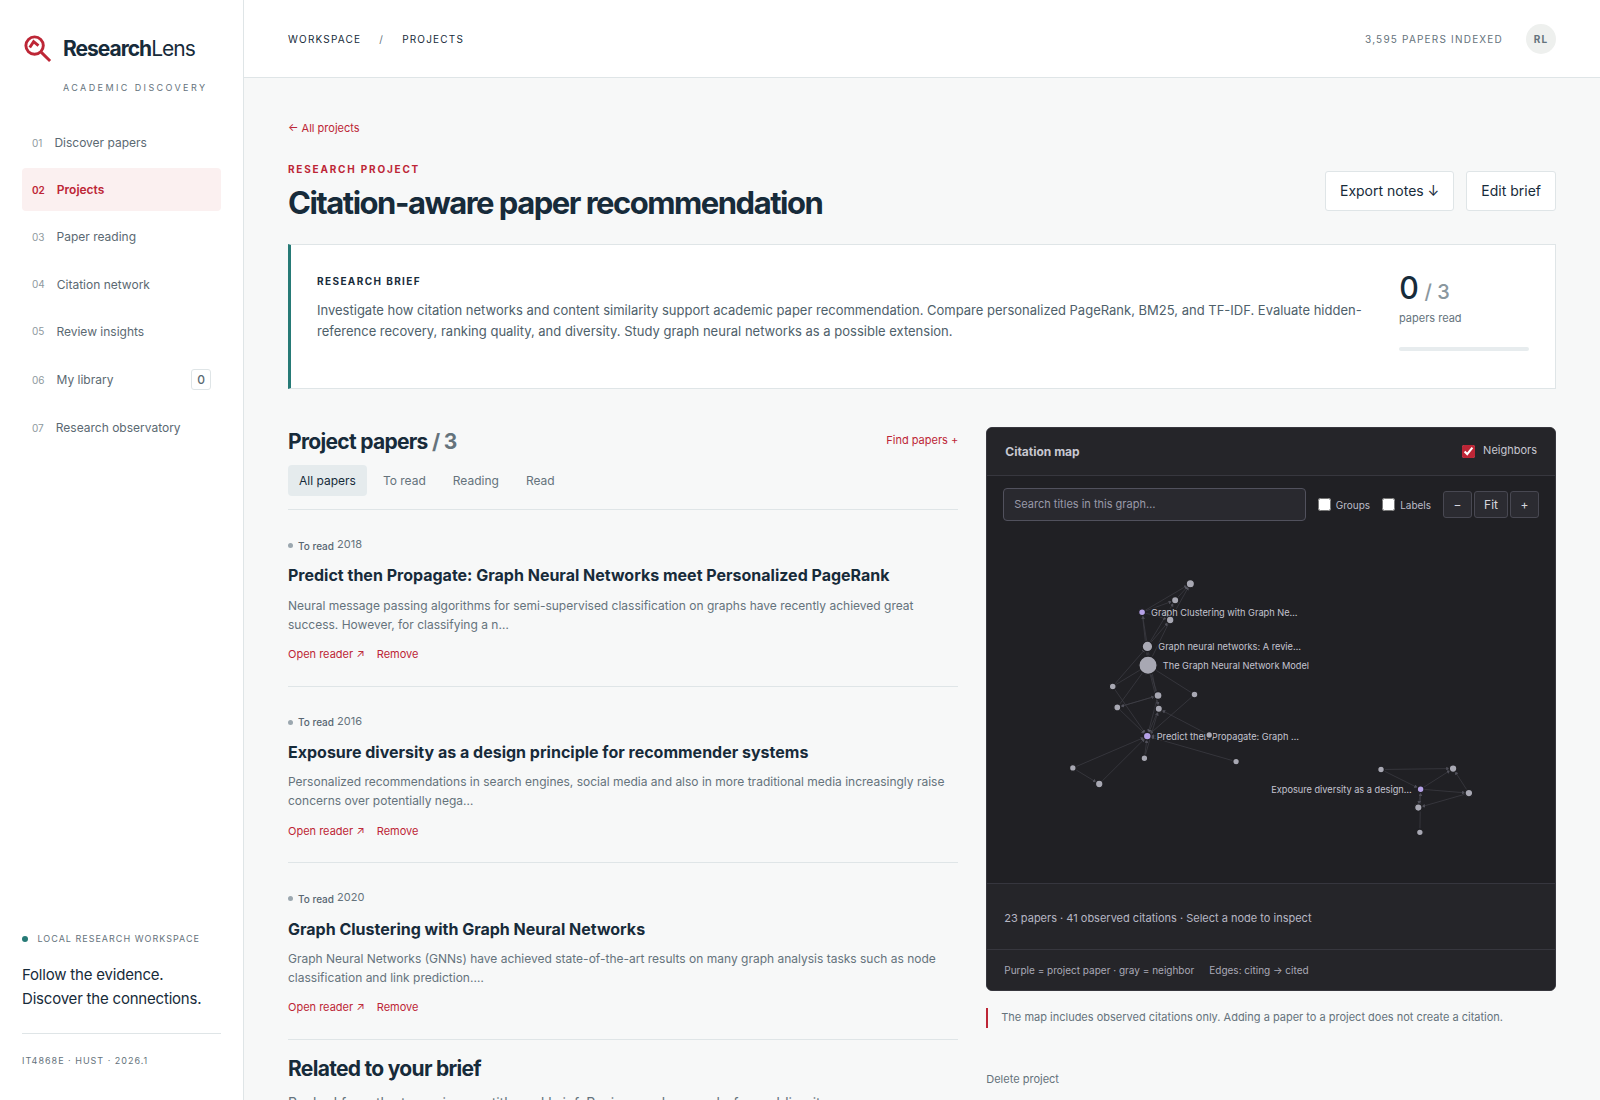
\includegraphics[width=\linewidth,height=5.4cm,keepaspectratio]{projects.png}
\column{.24\textwidth}\small\par\vspace{.25cm}
Brief dẫn truy hồi BM25.\par\vspace{.3cm}
Người đọc chọn paper và theo dõi tiến độ.\par\vspace{.3cm}
\takeaway{Membership không tạo citation mới.}
\end{columns}
\source{Ảnh browser QA; brief demo, paper và cạnh thật. Gợi ý theo brief chưa có benchmark relevance riêng.}
\end{frame}
\begin{frame}{Đọc PDF gốc cùng ghi chú và citation neighborhood}
\begin{columns}[T,onlytextwidth]
\column{.73\textwidth}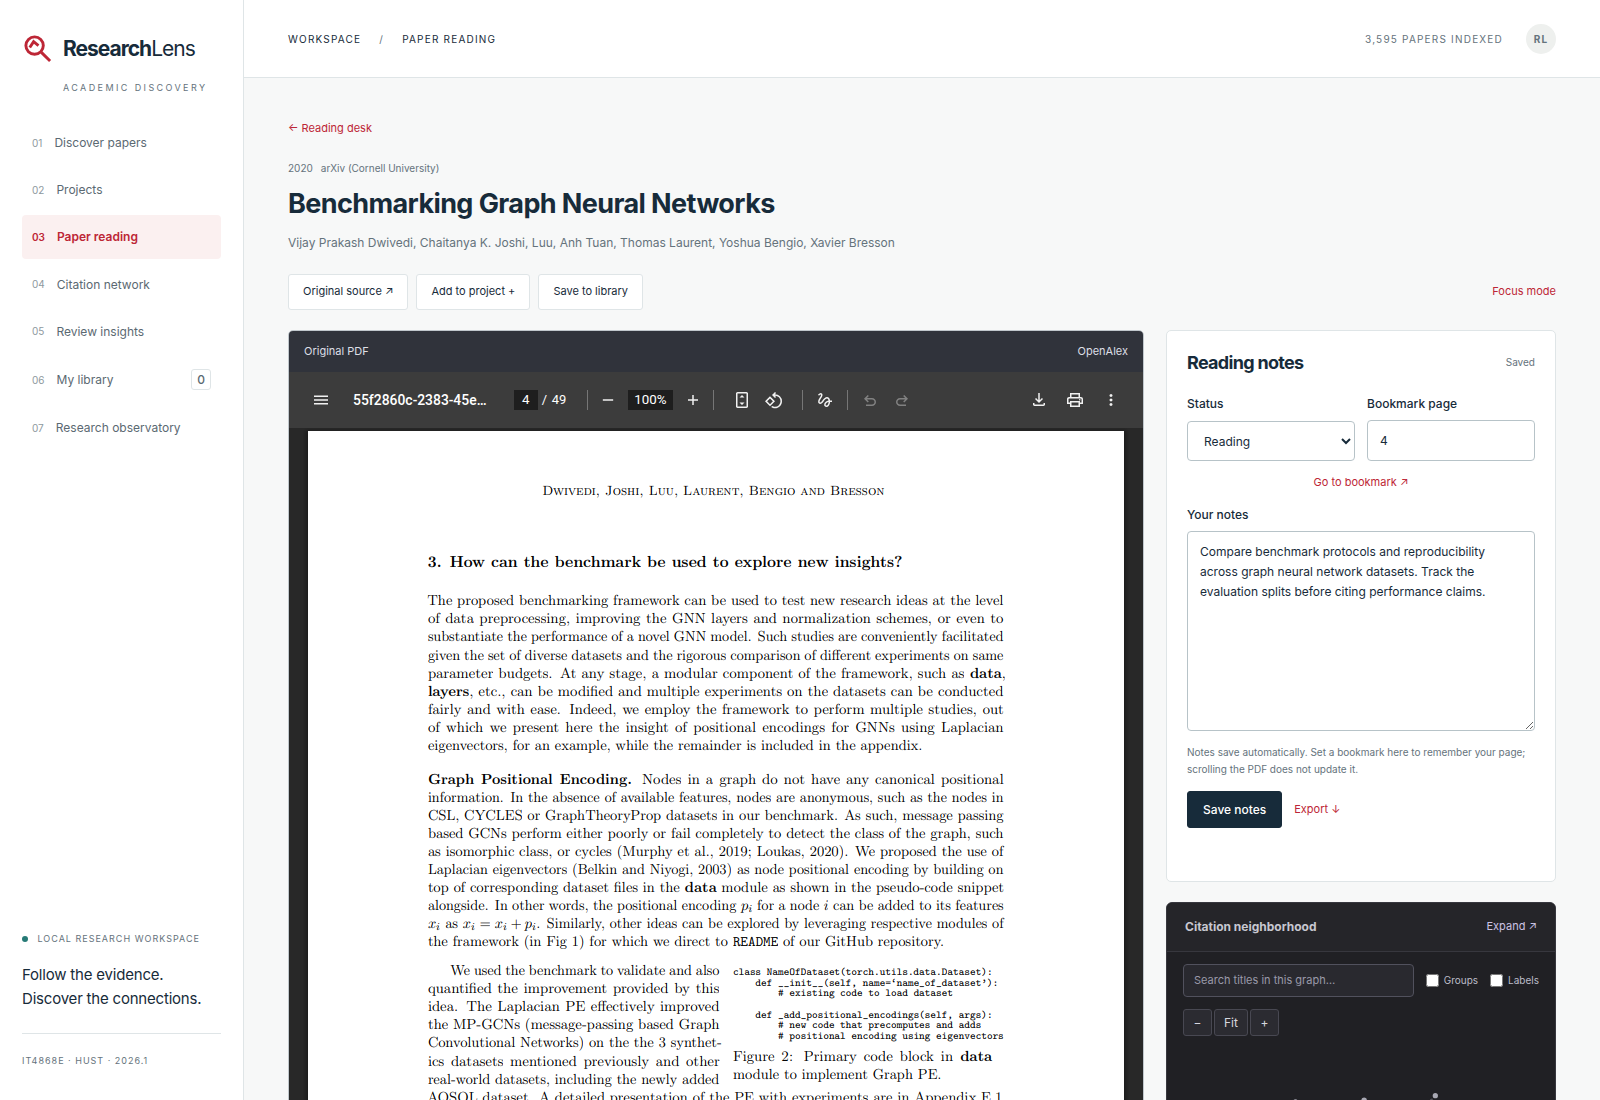
\includegraphics[width=\linewidth,height=5.4cm,keepaspectratio]{reading.png}
\column{.24\textwidth}\small\par\vspace{.25cm}
PDF thật từ repository.\par\vspace{.3cm}
Notes tự lưu; bookmark nhập tay.\par\vspace{.3cm}
\takeaway{PDF lỗi: abstract fallback được ghi rõ.}
\end{columns}
\source{Browser QA đã tải arXiv thật, thử notes UTF-8 >64 KiB và khôi phục draft. Graph hỗ trợ reduced motion.}
\end{frame}
\section{Thực nghiệm}
\begin{frame}{Mỗi tác vụ dùng một loại đáp án riêng}
\par\vspace{.15cm}
\small
\renewcommand{\arraystretch}{1.45}
\begin{tabular}{@{}p{3.5cm}p{4.4cm}p{5.1cm}@{}}\toprule
Tác vụ & Dữ liệu test & Chống leakage\\\midrule
Scientific retrieval & SciFact: 300 query / 5.183 abstracts & Qrels độc lập; không tune test\\
Gợi ý, thí nghiệm chính & 219 bài sau 2020; 826 reference che & Graph cắt ở 2020; bài test không có trong graph\\
Gợi ý, kiểm tra lại & 120 source papers; 442 cạnh che & Xóa toàn bộ cạnh test trước graph scoring\\
Review polarity & 115 review; official test split & Paper-disjoint; khử trùng; fit train-only\\\bottomrule
\end{tabular}
\par\vspace{.2cm}\takeaway{Bootstrap 95\% theo query/paper; không gộp thành một ``accuracy hệ thống''.}
\source{SciFact: Wadden et al. (2020), BEIR: Thakur et al. (2021); PeerRead: Kang et al. (2018). Seed 42.}
\end{frame}
\begin{frame}{Fusion dẫn đầu khi graph dừng ở năm 2020}
\begin{columns}[T,onlytextwidth]
\column{.44\textwidth}
\small Graph đến hết 2020: 2.520 bài, 7.881 cạnh. 219 bài test sau 2020, 826 reference bị che.\\[.2cm]
\textbf{RQ1} Đồng trích dẫn là tín hiệu đơn tốt nhất.\\[.1cm]
\textbf{RQ2} Fusion vượt hybrid +0,064 và vượt đồng trích dẫn +0,034.\\[.1cm]
\footnotesize Fusion được chọn sau khi xem E2. Split ngẫu nhiên ở slide sau cho kết quả ngược với đồng trích dẫn.
\column{.52\textwidth}
\small\begin{tabular}{lrr}\toprule
& nDCG@10 & Recall@10\\\midrule
Global PR & 0,032 & 0,058\\
Content & 0,110 & 0,147\\
PPR & 0,121 & 0,141\\
Hybrid (cũ) & 0,143 & 0,183\\
Đồng trích dẫn & 0,173 & 0,219\\
\textbf{Fusion (mới)} & \textbf{0,207} & \textbf{0,257}\\\bottomrule
\end{tabular}
\end{columns}
\source{Bootstrap ghép cặp 95\%: fusion -- hybrid [0,042; 0,087]; fusion -- đồng trích dẫn [0,016; 0,054]. Thắng/thua/hòa với hybrid 95/31/93. Nguồn: artifacts/temporal\_recovery.json.}
\end{frame}
\begin{frame}{Split ngẫu nhiên: đồng trích dẫn vẫn cao nhất}
\begin{columns}[T,onlytextwidth]
\column{.5\textwidth}
\par\vspace{.3cm}\small Split che ngẫu nhiên 120 bài, cố định từ trước\\[.3cm]
\begin{tabular}{lr}\toprule
& nDCG@10\\\midrule
Content & 0,070\\
Hybrid & 0,112\\
PPR & 0,174\\
Fusion & 0,259\\
Đồng trích dẫn & \textbf{0,305}\\\bottomrule
\end{tabular}
\column{.44\textwidth}
\par\vspace{.3cm}\small Fusion -- hybrid: +0,147\\
Fusion -- đồng trích dẫn: $-0{,}046$\\[.3cm]
Bỏ nhân chứng mới hơn bài nguồn: đồng trích dẫn chỉ giảm 0,305 xuống 0,301.\\[.3cm]
\takeaway{Fusion và đồng trích dẫn chưa phân xử được. Mặc định là fusion vì thắng thí nghiệm chính.}
\end{columns}
\source{scripts/evaluate\_holdout\_fusion.py; artifacts/holdout\_fusion.json. Khoảng 95\% fusion -- đồng trích dẫn [$-0{,}083$; $-0{,}007$].}
\end{frame}
\begin{frame}{Phép thử gần thực tế hơn: tác giả đọc gì tiếp}
\begin{columns}[T,onlytextwidth]
\column{.40\textwidth}
\small Thư viện là bài của tác giả đến 2020 và reference của chúng. Đáp án là bài họ trích \textbf{lần đầu} sau 2020.\\[.2cm]
250 tác giả, 1.899 đáp án.\\[.2cm]
Hồi quy logistic trên 8 tín hiệu có tên, huấn luyện ở mốc 2018.\\[.2cm]
\footnotesize Che reference có lợi sẵn cho tín hiệu trích dẫn. Phép thử này bớt lợi thế đó.
\column{.56\textwidth}
\scriptsize\begin{tabular}{lrrrr}\toprule
& \multicolumn{2}{c}{Che reference} & \multicolumn{2}{c}{Tác giả}\\
& nDCG & Hit & nDCG & Hit\\\midrule
Global PR & 0,032 & 0,18 & 0,047 & 0,31\\
Content & 0,110 & 0,37 & 0,068 & 0,22\\
Hybrid & 0,143 & 0,42 & 0,070 & 0,24\\
Đồng trích dẫn & 0,173 & 0,53 & 0,099 & 0,40\\
Fusion & 0,207 & 0,58 & 0,113 & 0,42\\
\textbf{Hồi quy logistic} & \textbf{0,231} & \textbf{0,66} & \textbf{0,136} & \textbf{0,45}\\\bottomrule
\end{tabular}\par\vspace{.2cm}
\takeaway{Tác giả thật đọc bài mới và nổi tiếng. Độ mới và số trích dẫn có trọng số lớn nhất.}
\end{columns}
\source{Hit = có ít nhất một đáp án trong top 10. Logistic -- fusion: +0,023 [0,006; 0,040] và +0,022 [0,007; 0,040]. Nguồn: artifacts/author\_next.json, artifacts/ltr.json.}
\end{frame}
\chartslide{Trong 5 cách cũ, PPR dẫn đầu khi che cạnh ngẫu nhiên}{slide_recommendation.pdf}{\bigmetric{0,174}{nDCG@10 của PPR}\par\vspace{.4cm}\small Hybrid: 0,112\par Content: 0,063\par\vspace{.35cm}\par\takeaway{Hybrid chưa thắng graph-only.}}{120 source papers; toàn corpus làm ứng viên, loại seed/source. Error bars: 2.000 bootstrap samples. Nguồn: artifacts/results.json.}
\chartslide{Hybrid cải thiện content với hiệu ghép cặp dương}{slide_diversity.pdf}{\bigmetric{+0,049}{nDCG: hybrid -- content}\par\vspace{.3cm}\small CI 95\%:\par [0,027; 0,073]\par\vspace{.3cm}\par MMR tăng diversity và coverage của hybrid.}{Hiệu ghép cặp theo cùng source paper. Diversity = 1 -- mean cosine; bubble area theo coverage. Nguồn: artifacts/results.json.}
\chartslide{Review polarity còn khó dù có tín hiệu học được}{slide_opinion.pdf}{\bigmetric{0,469}{macro-F1 của logreg}\par\vspace{.3cm}\small Lexicon: 0,436\par Majority: 0,181\par\vspace{.3cm}\par\takeaway{CI chồng lấn; chưa khẳng định hơn lexicon.}}{115 test reviews. Cluster bootstrap theo paper, 1.000 samples. Nhãn suy từ rating. Nguồn: PeerRead + artifacts/results.json.}
\chartslide{BM25 cải thiện nDCG nhưng recall không tăng}{slide_retrieval.pdf}{\bigmetric{0,651}{nDCG@10 của BM25}\par\vspace{.35cm}\small TF-IDF: 0,621\par\vspace{.3cm}\par Recall@10:\par BM25 0,768\par TF-IDF 0,778}{SciFact test (300 queries); benchmark sparse local, không phải số đo Solr. Nguồn: Wadden et al. (2020); artifacts/results.json.}
\chartslide{Warm local search hoàn thành trong vài mili giây}{slide_latency.pdf}{\small 8 query × 10 lần\par CPU, single process\par\vspace{.4cm}\takeaway{Không gồm HTTP/browser hoặc tải đồng thời.}\par\vspace{.4cm}\small Artifact lưu môi trường và phiên bản.}{Scope: filtering + scoring + ranking + top-20 serialization. Thời gian phụ thuộc máy. Nguồn: artifacts/results.json.}

\section{Kiểm chứng và kết luận}
\begin{frame}{Audit và test độc lập phát hiện lỗi trước bàn giao}
\begin{columns}[T,onlytextwidth]
\column{.31\textwidth}\par\vspace{.5cm}\bigmetric{441/441}{test tự động đạt}\par\vspace{.4cm}\small Package ứng dụng đạt 99\% statement coverage.
\column{.61\textwidth}\par\vspace{.3cm}
\textbf{Các lỗi đã sửa}\par
JSONL có line separator Unicode.\par
Seed bị cắt ở 50; saved IDs cũ.\par
Lưu notes UTF-8 dài; modal race.\par
Alias citation; parser program cũ.
\par\vspace{.25cm}\takeaway{Browser demo và Docker Solr đã chạy trực tiếp.}
\end{columns}
\source{docs/AUDIT.md; docs/TEST\_REPORT.md; artifacts/browser\_qa.json; artifacts/solr\_integration.json. Coverage không chứng minh không còn lỗi.}
\end{frame}
\begin{frame}{Proxy evaluation chưa thay thế nghiên cứu người dùng}
\par\vspace{.4cm}
\begin{columns}[T,onlytextwidth]
\column{.46\textwidth}\textbf{Giới hạn hiện tại}\par Reference recovery có lợi sẵn cho trích dẫn.\par Fusion và đồng trích dẫn chưa phân xử được.\par Tác giả trùng tên bị gộp.\par Gợi ý theo brief chưa có người chấm.
\column{.46\textwidth}\textbf{Bước kiểm chứng tiếp}\par SPECTER2 thay TF-IDF.\par Kiểm tra hồi quy logistic trên E3.\par Người đọc chấm 43 cặp brief--paper.\par Annotation aspect cho review.
\end{columns}
\par\vspace{.7cm}\takeaway{770 isolates và missing abstracts ảnh hưởng kết quả.}
\source{Phân tích giới hạn từ snapshot và protocol đã thực thi; chưa có user study hoặc A/B test.}
\end{frame}
\begin{frame}{Các phương pháp và dữ liệu có nguồn truy xuất}
\fontsize{8}{11}\selectfont
\begin{columns}[T,onlytextwidth]
\column{.48\textwidth}
\textbf{Retrieval và graph}\par
Manning, Raghavan, Schütze (2008). \emph{Introduction to Information Retrieval}. CUP.\par
Robertson, Zaragoza (2009). \emph{The Probabilistic Relevance Framework: BM25 and Beyond}. FnT IR 3(4), 333--389.\par
Page et al. (1999). \emph{The PageRank Citation Ranking}. Stanford InfoLab.\par
Kleinberg (1999). \emph{Authoritative Sources in a Hyperlinked Environment}. JACM 46(5), 604--632.\par
Blondel et al. (2008). \emph{Fast Unfolding of Communities in Large Networks}. JSTAT P10008.
\column{.48\textwidth}
\textbf{Diversity và datasets}\par
Carbonell, Goldstein (1998). \emph{The Use of MMR, Diversity-Based Reranking}. SIGIR, 335--336.\par
Kang et al. (2018). \emph{A Dataset of Peer Reviews (PeerRead)}. NAACL, 1647--1661.\par
Wadden et al. (2020). \emph{Fact or Fiction: Verifying Scientific Claims}. EMNLP, 7534--7550.\par
Thakur et al. (2021). \emph{BEIR: A Heterogeneous Benchmark}. NeurIPS Datasets and Benchmarks.\par
OpenAlex API; Apache Solr 9.9 Reference Guide. Truy cập 14/10/2026.
\end{columns}
\source{DOI/URL đầy đủ ở report/references.bib. Toàn bộ chart là kết quả đo của dự án; screenshot là bản chạy thật.}
\end{frame}
\begin{frame}{Tín hiệu trích dẫn quyết định gợi ý bài đọc tiếp}
\par\vspace{.25cm}
{\Large\bfseries Ba kết luận từ bản chạy}\par\par\vspace{.4cm}
\textbf{01}\quad Đồng trích dẫn là tín hiệu đơn tốt nhất trên cả ba protocol.\par\par\vspace{.18cm}
\textbf{02}\quad Fusion vượt hybrid trên cả ba protocol. Hồi quy logistic còn thêm khoảng +0,02.\par\par\vspace{.18cm}
\textbf{03}\quad Review model cần đi cùng evidence và giới hạn.
\par\vspace{.6cm}
\takeaway{Demo: \url{http://127.0.0.1:8765}}\par
{\small Tái lập: README.md\quad |\quad kết quả: artifacts/temporal\_recovery.json}
\source{ResearchLens · IT4868E · HUST. Bản bàn giao có source, snapshot, tests, LaTeX và HUST Beamer.}
\end{frame}
\appendix
\section{Phụ lục}
\begin{frame}{Phụ lục A: Che cạnh trước mọi phép tính graph}
\par\vspace{.3cm}
\begin{enumerate}
\item Chọn source có ít nhất 6 local references.
\item Che $\lfloor m/3\rfloor$ references của từng source.
\item Xóa hợp tất cả cạnh test: 442 cạnh.
\item Recompute graph scores trên 13.039 cạnh còn lại.
\item Dùng references còn lại làm seed; loại source/seed.
\end{enumerate}
\par\vspace{.4cm}\takeaway{Paper test còn là node: đây là transductive evaluation.}
\source{Split cụ thể: artifacts/recommendation\_split.jsonl; SHA-256 lưu trong artifacts/results.json.}
\end{frame}
\begin{frame}{Phụ lục B: Nhãn mixed dễ nhầm với cả hai phía}
\begin{columns}[T,onlytextwidth]\column{.67\textwidth}\includegraphics[width=\linewidth,height=5.3cm,keepaspectratio]{confusion.pdf}\column{.29\textwidth}\par\vspace{.4cm}\small Một review có thể khen cách viết nhưng chê đóng góp.\par\vspace{.4cm}\par Điểm reviewer phản ánh nhiều khía cạnh.\par\vspace{.4cm}\par\takeaway{Không dùng prediction để kết luận accept/reject.}\end{columns}
\source{Logistic regression, test split PeerRead ICLR 2017. Ma trận lấy trực tiếp từ results.json.}
\end{frame}
\begin{frame}{Phụ lục C: Evidence nối review với khía cạnh cụ thể}
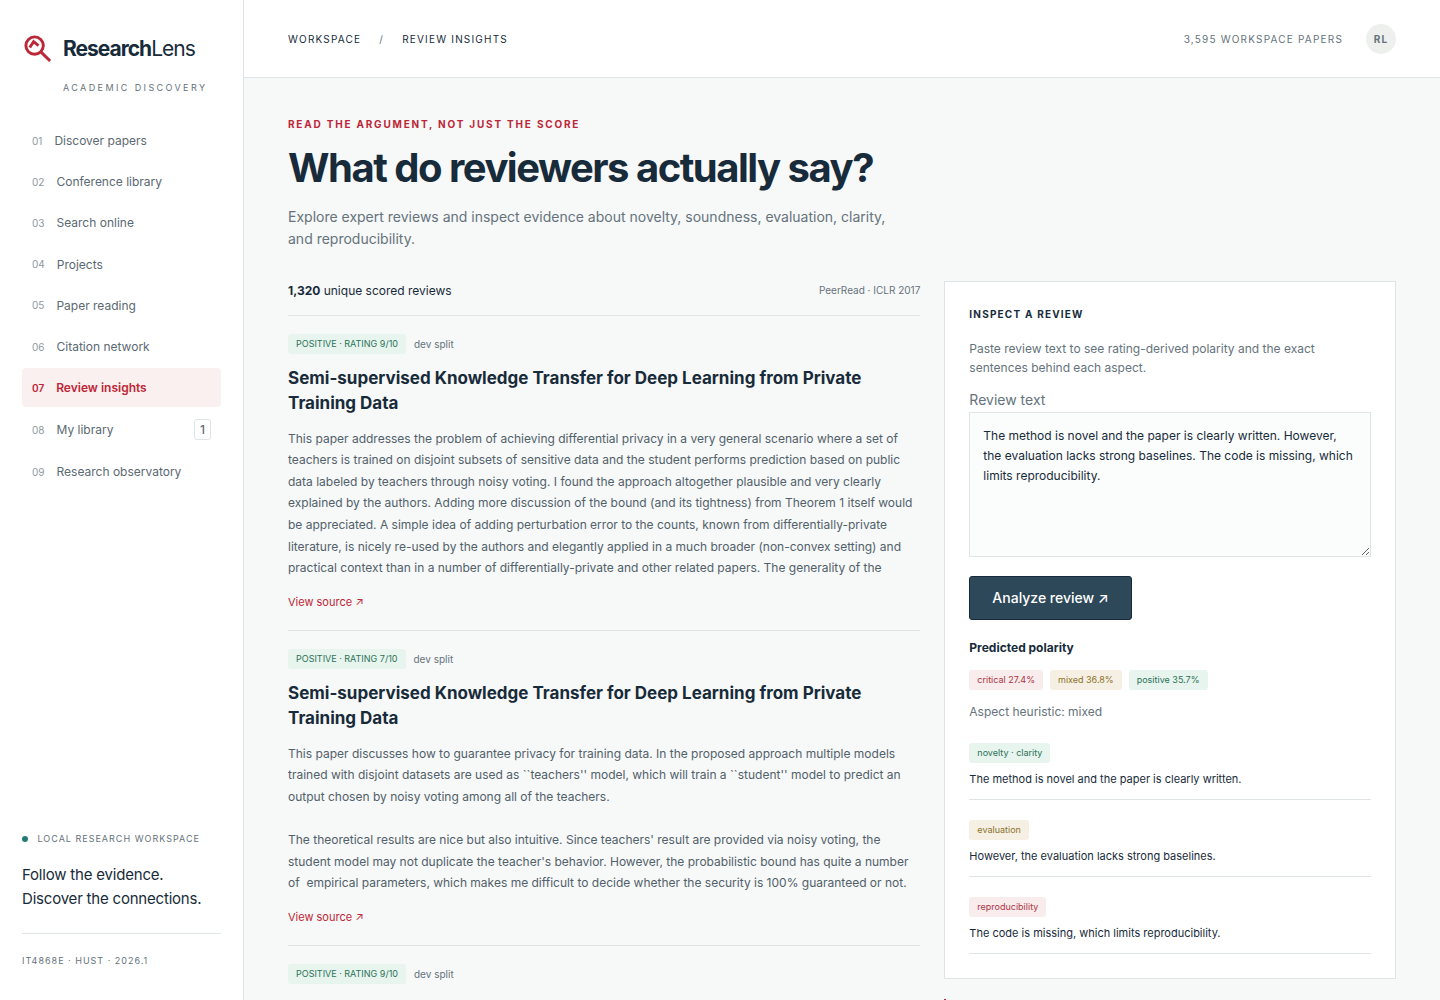
\includegraphics[width=\textwidth,height=5.6cm,keepaspectratio]{reviews.png}
\source{Ảnh giao diện thật. Review phía trái lấy từ PeerRead; đoạn nhập phía phải là ví dụ demo, không dùng trong benchmark.}
\end{frame}
\begin{frame}{Phụ lục D: Thí nghiệm thăm dò cho chức năng Reader}
\par\vspace{.4cm}
Tìm bài từ một câu trong abstract thuộc truy hồi, không thuộc RQ1 và RQ2.\par\vspace{.3cm}
Mỗi phép đo có 9 đến 172 truy vấn, khoảng tin cậy rộng.\par\vspace{.3cm}
\takeaway{Chỉ dùng để chọn cấu hình mặc định cho Reader.}
\source{CSFCube, SciERC, ACL-ARC. Chi tiết ở Phụ lục B của báo cáo.}
\end{frame}
\chartslide{Thêm Laya cải thiện thứ hạng ở 2 trong 9 truy vấn}{decision_by_query.pdf}{\bigmetric{0,365}{nDCG@10 với TF-IDF + MiniLM}\par\vspace{.34cm}\small Thêm Laya: 0,339.\par\vspace{.30cm}\small Mỗi thanh là một bài mẫu. Thanh bên phải mốc 0 biểu thị top 10 tốt hơn.}{CSFCube, phần phương pháp (Mysore và cộng sự, 2021). 1.218 cặp test do chuyên gia chấm. Chênh lệch trung bình $-0{,}026$, khoảng bootstrap 95\% [$-0{,}056$, $+0{,}007$].}

\chartslide{Từ một câu trong abstract đến ba bài đọc tiếp}{passage_reader.png}{\bigmetric{8/27}{vị trí top 3 có bài cùng phương pháp, theo nhãn chuyên gia}\par\vspace{.28cm}\small Người đọc chọn câu. Hệ thống xếp hạng bài và đưa ra câu trích để đối chiếu.}{Ảnh giao diện thực. CSFCube, Mysore và cộng sự (2021), 9 truy vấn phương pháp. Phương án phối hợp độ giống câu và abstract đạt 6/27.}

\begin{frame}{ASPIRE cải thiện top 3 trên nhóm bài mẫu mới}
\par\vspace{.4cm}
\begin{columns}[T,onlytextwidth]\column{.64\textwidth}
\small Số vị trí hữu ích trong ba bài đầu, theo chuyên gia\\[.2cm]
\begin{tabular}{@{}lrr@{}}\toprule
Truy vấn & Reader & ASPIRE\\\midrule
Phương pháp đã đo & 8/27 & 7/27\\
Kết quả đã đo & 8/18 & 10/18\\
Bối cảnh, kết quả trên bài mới & 19/42 & \textbf{24/42}\\\bottomrule
\end{tabular}
\column{.31\textwidth}\bigmetric{+11,9}{điểm phần trăm precision@3 trên 14 tác vụ chuyển giao}
\par\vspace{.35cm}\small Reader giữ mô hình hiện tại vì top 3 ở nhóm phương pháp giảm.
\end{columns}
\source{CSFCube. Chọn trọng số trên 8 truy vấn phương pháp. Tập chuyển giao gồm 11 bài mẫu riêng biệt. Khoảng bootstrap ghép cặp 95\% cho chênh lệch precision@3 xấp xỉ [0,0; 25,0] điểm phần trăm.}
\end{frame}

\chartslide{Tên kỹ thuật giúp tìm đúng bài trong top 3}{method_name_ablation.pdf}{\bigmetric{+8,1}{điểm phần trăm khi giữ tên kỹ thuật}\par\vspace{.3cm}\small 23 câu tìm thấy thêm bài đúng, 9 câu mất bài đúng.}{SciERC (Luan và cộng sự, 2018). Mỗi câu tìm trong 499 abstract. Nhãn đúng là cùng tên phương pháp đã được đánh dấu. Khoảng bootstrap 95\% theo 81 tên [2,6; 14,0] điểm phần trăm.}

\begin{frame}{Mười hai nguồn cần tìm đã vắng mặt ở top 20}
\par\vspace{.4cm}
\begin{columns}[T,onlytextwidth]
\column{.46\textwidth}\bigmetric{14/26}{câu trích dùng có nguồn đúng trong 20 ứng viên}
\column{.48\textwidth}\small Số câu còn nguồn đúng trong top 3\\[.18cm]
\begin{tabular}{@{}lr@{}}\toprule
Giữ thứ tự fusion & 8/26\\
Laya chấm mức khớp kỹ thuật & 6/26\\
Cross-encoder MS MARCO & 4/26\\\bottomrule
\end{tabular}
\end{columns}
\par\vspace{.45cm}\takeaway{Để tìm lại 12 nguồn còn thiếu, cần cải thiện bước lấy ứng viên.}
\source{ACL-ARC, 26 câu Uses thuộc 21 bài nguồn. Chỉ có tiêu đề ứng viên. Cả hai mô hình xếp lại cùng top 20. Khoảng 95\% của Laya so với fusion [$-22{,}2$; $+7{,}7$] điểm phần trăm.}
\end{frame}

\begin{frame}{Phụ lục E: Demo theo một luồng đọc có thể lặp lại}
\par\vspace{.35cm}
\begin{enumerate}
\item Tìm ``graph neural networks''; đổi ranking/filter.
\item Mở paper, kiểm tra nguồn và lưu vào library.
\item Mở citation neighborhood; chỉ hướng cạnh.
\item Gợi ý mặc định fusion; mở bài nhân chứng; so với hybrid; xuất BibTeX.
\item Xem review evidence và dashboard thực nghiệm.
\end{enumerate}
\source{Sau phụ lục, quay về slide kết luận khi thảo luận. File metadata chung: report/metadata.tex.}
\end{frame}
\end{document}
